\section{Introduction}
%----------------------------------------------------------------------
%----------------------------------------------------------------------
\begin{frame}[c]{Global Optimization}
Consider a 'well behaved' function $\cost$ : $\pcs \rightarrow \realnum$ where $\pcs \subseteq \realnum^D$ is a bounded domain.
\begin{equation*}
  \conf=\argmin_{\conf\in\pcs} \cost(\conf) 
\end{equation*}
\begin{figure}
   \begin{multicols}{2}
    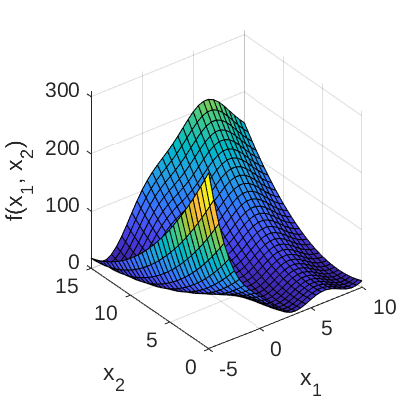
\includegraphics[width=0.2\textwidth, right]{w06_hpo_bo/images/intro_images/branin.png}
    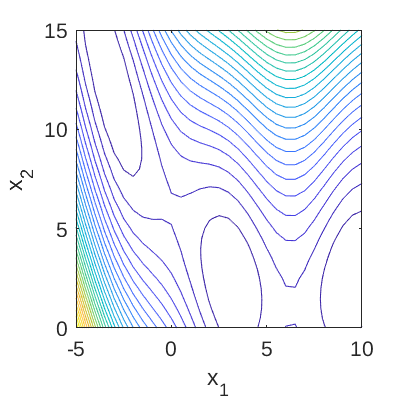
\includegraphics[width=0.2\textwidth,left]{w06_hpo_bo/images/intro_images/branin_countour.png}
 \end{multicols}
\end{figure}
\begin{itemize}
    \item Function $\cost$ is explicitly unknown and multimodal
    \item Only interaction: Query of function $\conf$ to obtain $\cost(\conf)$
    \item Evaluations of $\cost$ may be noisy
    \item Evaluations of $\cost$ are expensive
\end{itemize}

\tiny{\source{https://uqworld.org/} }


\end{frame}

%----------------------------------------------------------------------
%----------------------------------------------------------------------
%\begin{frame}[c]{Optimization problem example}

%We know that:
%\begin{itemize}
%    \item The function $\cost$ is Lipschitz continuous and differentiable.
%    \pause
%    \item The minimizer of $\cost$ is in the interval [0,1].
%    \pause
%    \item We have observed 3 evaluations of $\cost$.
%\end{itemize}

%\end{frame}
%----------------------------------------------------------------------
%\begin{frame}[c]{Problem description}
%\framesubtitle{We have 4 function evaluations}
%\begin{figure}
%    \centering
%    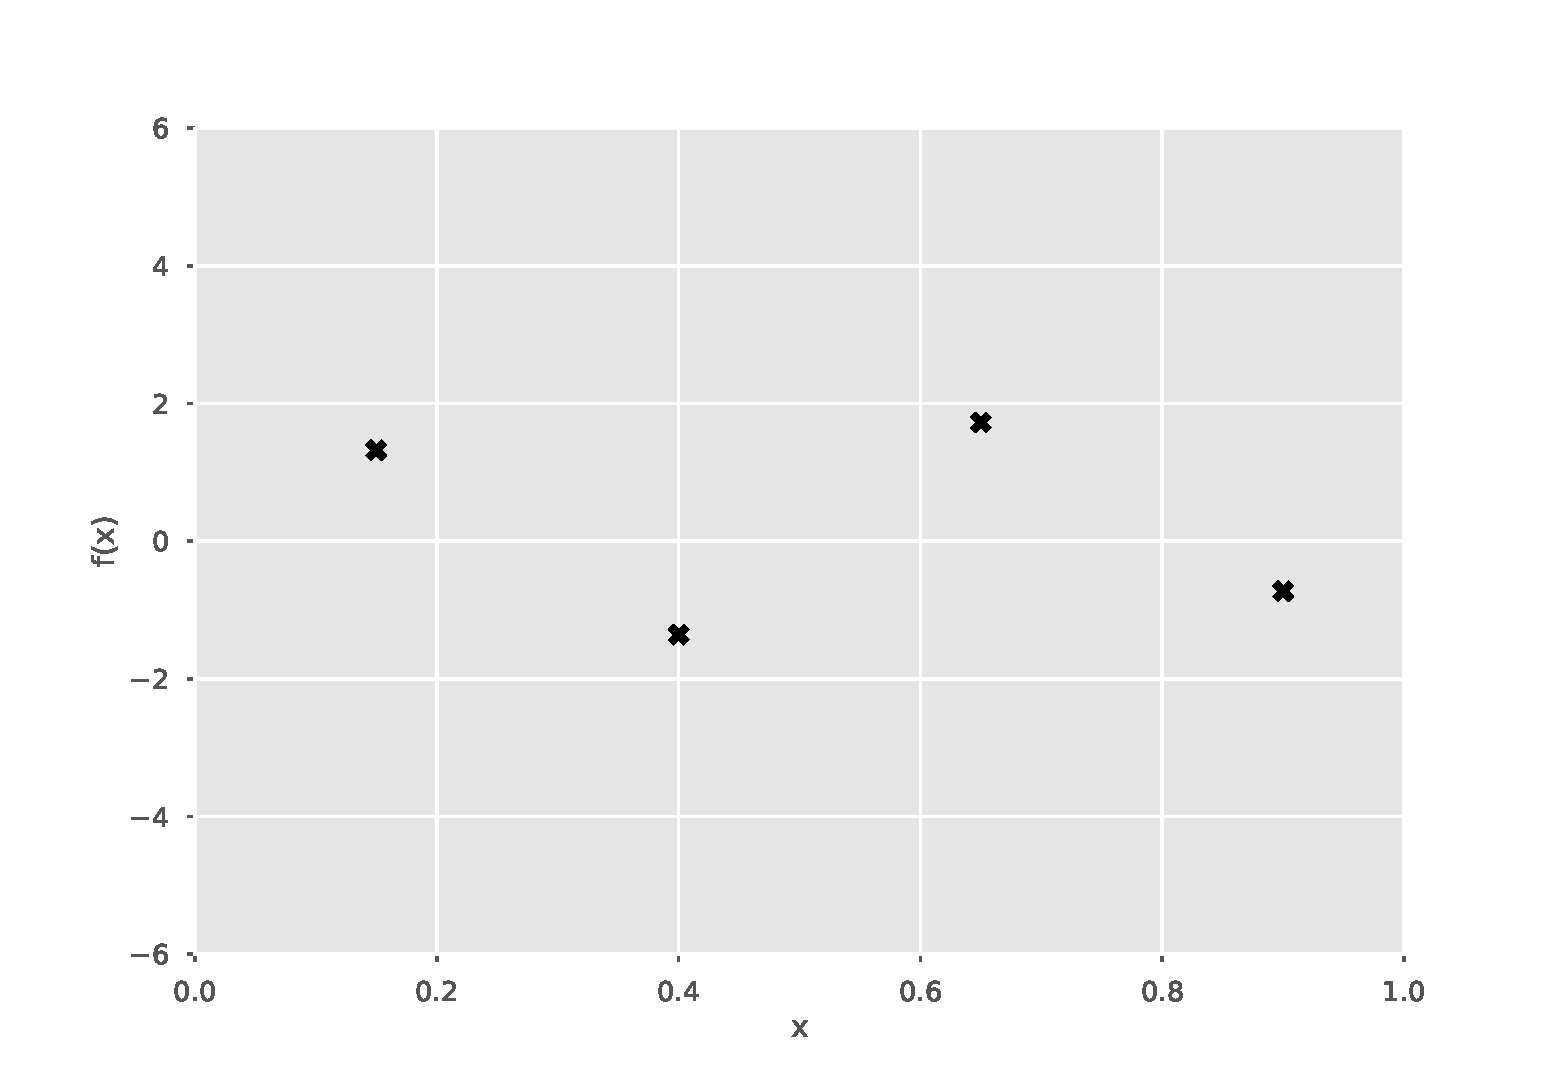
\includegraphics[width=0.8\textwidth, %height=0.38\textwidth]{w06_hpo_bo/images/intro_images/plot_datapoints.p%df}
%    \label{fig:my_label}
%\end{figure}
%\begin{center}
%  Where is the minimum of function $f$?  
%\end{center}
%\source{Plots are based on Javier Gonz\'alez's BO lecture %(bo\_intro.py)}



%\end{frame}

%-----------------------------------------------------------------------
%----------------------------------------------------------------------
%\begin{frame}[c]{Problem description}
%\framesubtitle{One possible curve}
%\begin{figure}
%    \centering
%    \includegraphics[width=0.7\textwidth, %height=0.4\textwidth]{w06_hpo_bo/images/intro_images/plot_posterior_1_s%ample.pdf}
%    \label{fig:my_label}
%\end{figure}
%\source{Plots are based on Javier Gonz\'alez's BO lecture %(bo\_intro.py)}



%\end{frame}

%-----------------------------------------------------------------------
%----------------------------------------------------------------------
%\begin{frame}[c]{Problem description}
%\framesubtitle{Three possible curves}
%\begin{figure}
%    \centering
%    \includegraphics[width=0.7\textwidth, %height=0.4\textwidth]{w06_hpo_bo/images/intro_images/plot_posterior_3_s%ample.pdf}
%    \label{fig:my_label}
%\end{figure}
%\source{Plots are based on Javier Gonz\'alez's BO lecture %(bo\_intro.py)}



%\end{frame}

%-----------------------------------------------------------------------
%----------------------------------------------------------------------
%\begin{frame}[c]{Problem description}
%\framesubtitle{Ten possible curves}
%\begin{figure}
%    \centering
%    \includegraphics[width=0.7\textwidth, %height=0.4\textwidth]{w06_hpo_bo/images/intro_images/plot_posterior_10_%sample.pdf}
%    \label{fig:my_label}
%\end{figure}
%\source{Plots are based on Javier Gonz\'alez's BO lecture %(bo\_intro.py)}



%\end{frame}

%-----------------------------------------------------------------------
%----------------------------------------------------------------------
%\begin{frame}[c]{Problem description}
%\framesubtitle{One hundred possible curves}
%\begin{figure}
%    \centering
%    \includegraphics[width=0.7\textwidth, %height=0.4\textwidth]{w06_hpo_bo/images/intro_images/plot_posterior_100%_sample.pdf}
%    \label{fig:my_label}
%\end{figure}
%\source{Plots are based on Javier Gonz\'alez's BO lecture %(bo\_intro.py)}



%\end{frame}

%-----------------------------------------------------------------------%----------------------------------------------------------------------
%\begin{frame}[c]{Problem description}
%\framesubtitle{One thousand possible curves}
%\begin{figure}
%    \centering
%    \includegraphics[width=0.7\textwidth, %height=0.4\textwidth]{w06_hpo_bo/images/intro_images/plot_posterior_100%0_sample.pdf}
%    \label{fig:my_label}
%\end{figure}
%\source{Plots are based on Javier Gonz\'alez's BO lecture (bo\_intro.py)}



%\end{frame}

%-----------------------------------------------------------------------
%----------------------------------------------------------------------
%\begin{frame}[c]{Problem description}
%\framesubtitle{Infinitely many curves}
%\begin{figure}
%    \centering
%    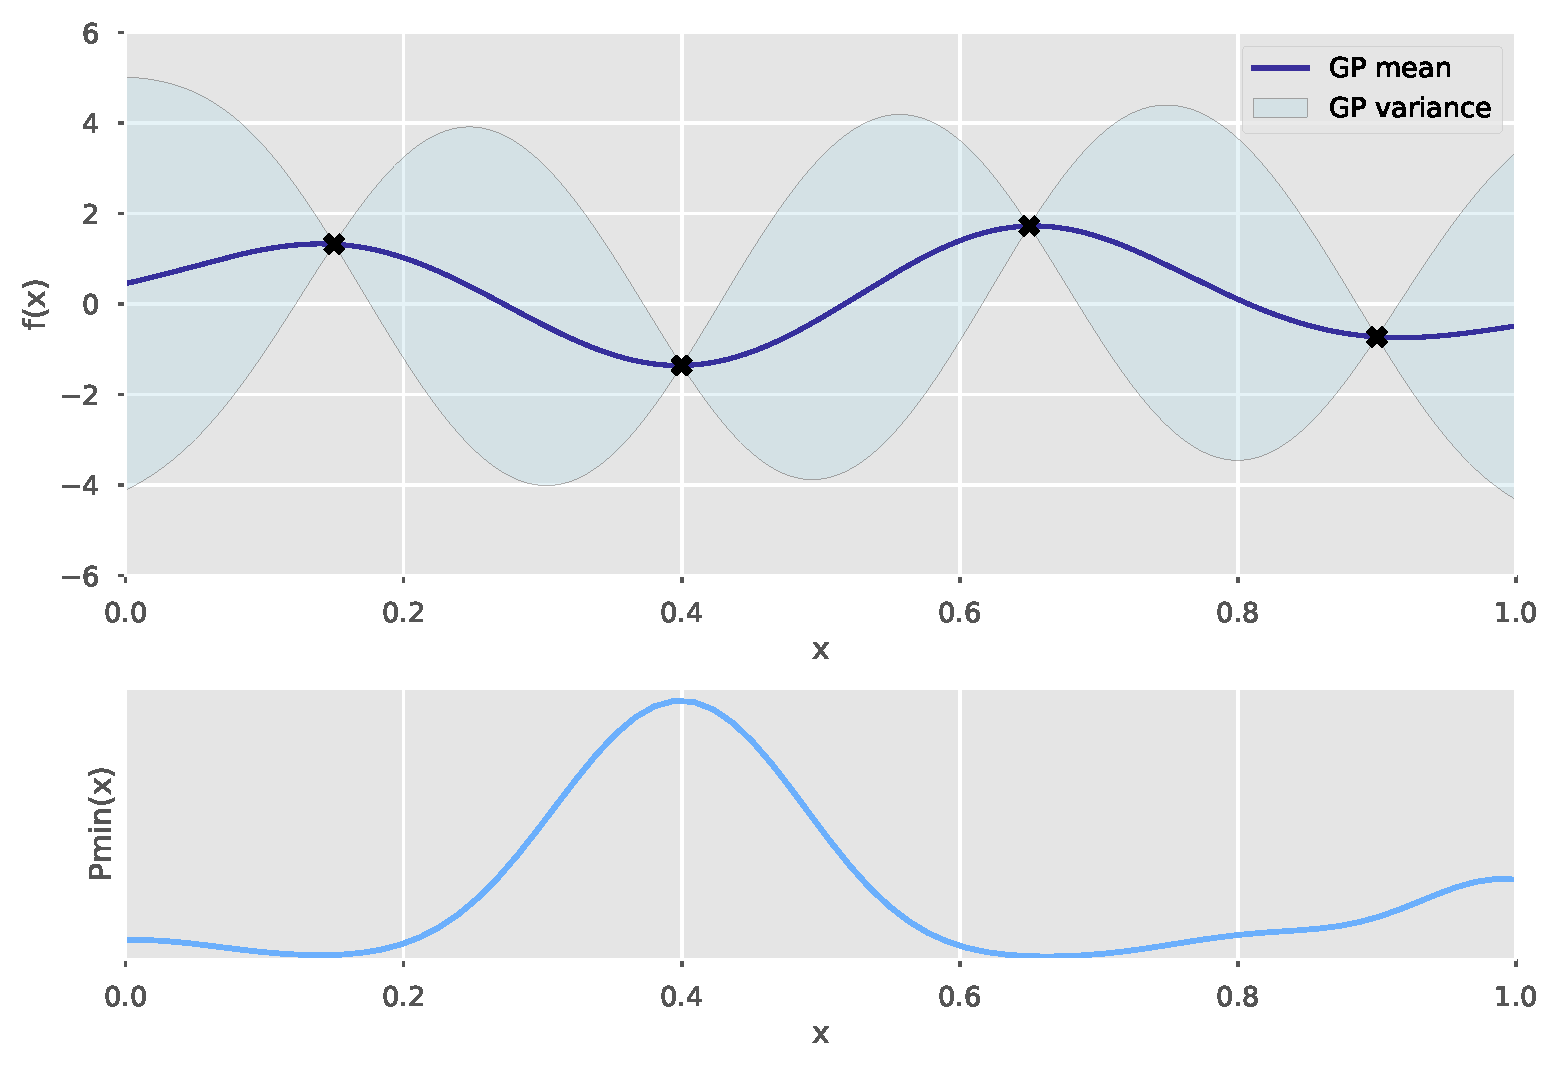
\includegraphics[width=0.7\textwidth, %height=0.4\textwidth]{w06_hpo_bo/images/intro_images/plot_posterior.pdf%}
%    \label{fig:my_label}
%\end{figure}
%\source{Plots are based on Javier Gonz\'alez's BO lecture (bo\_intro.py)}


%\end{frame}

%-----------------------------------------------------------------------
%----------------------------------------------------------------------
\begin{frame}[c]{Problem description}
\begin{figure}
    \centering
    \only<1>{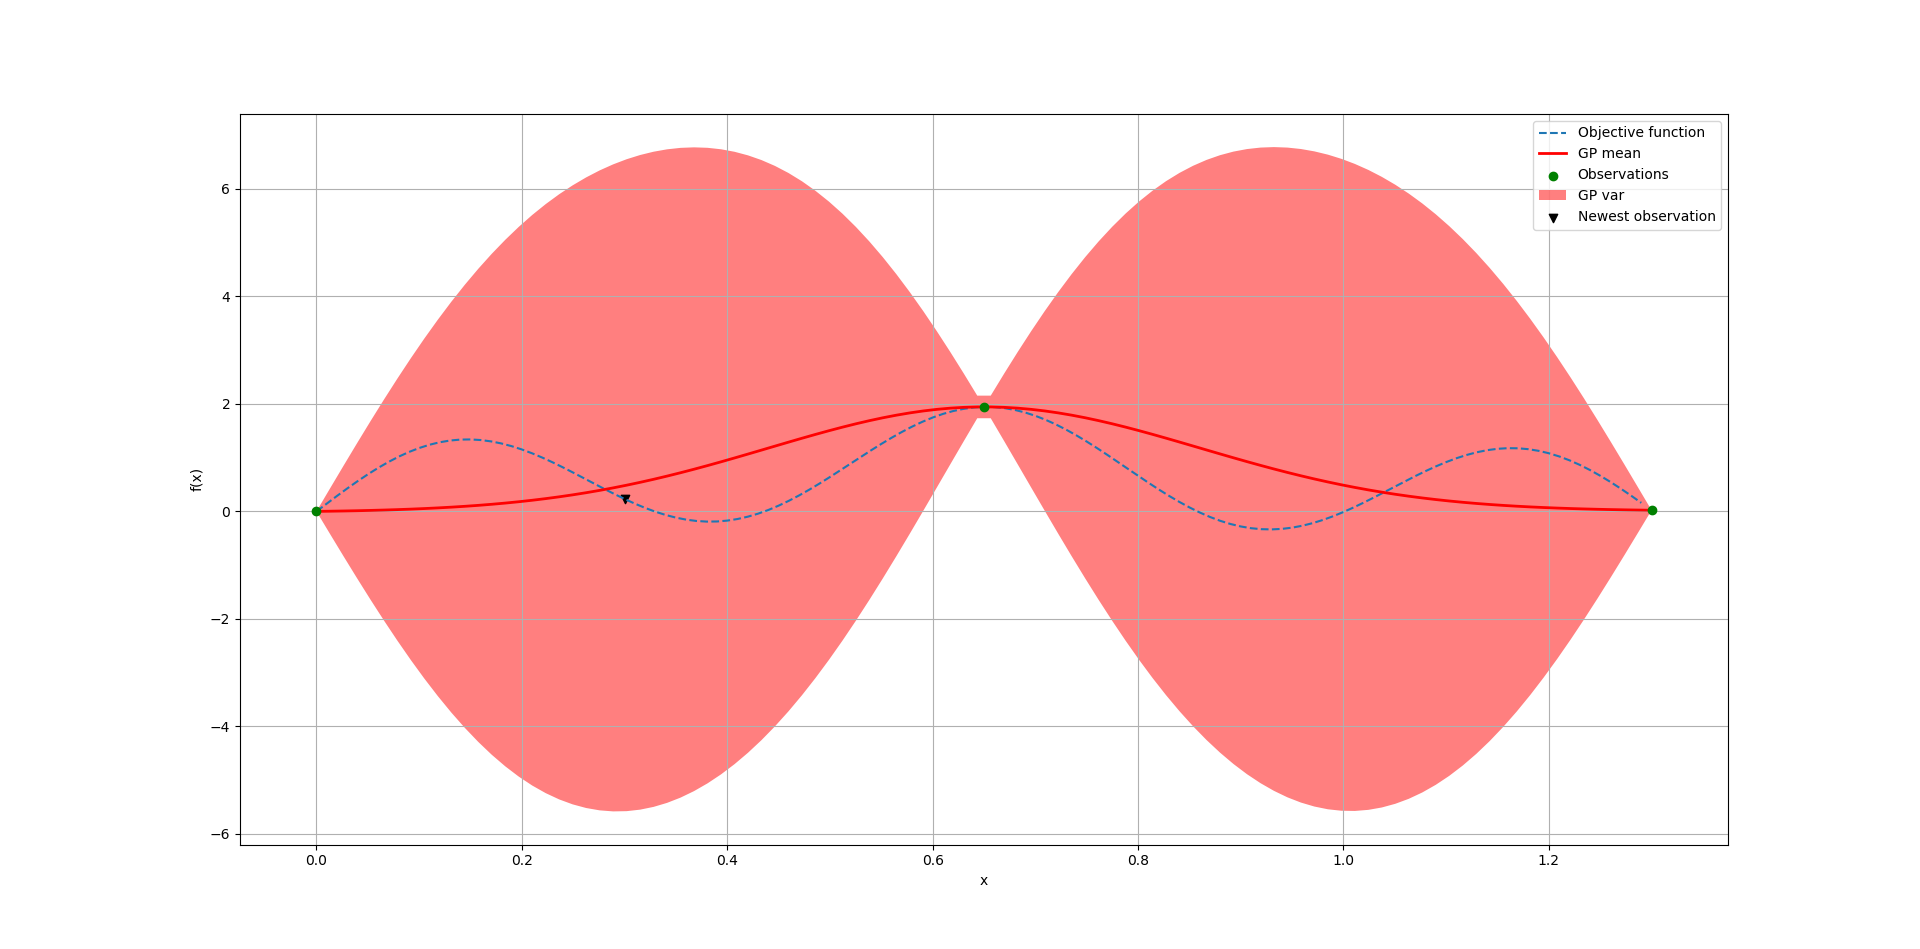
\includegraphics[width=\linewidth]{w06_hpo_bo/images/intro_images/BOLoop_1.png}}
    \only<2>{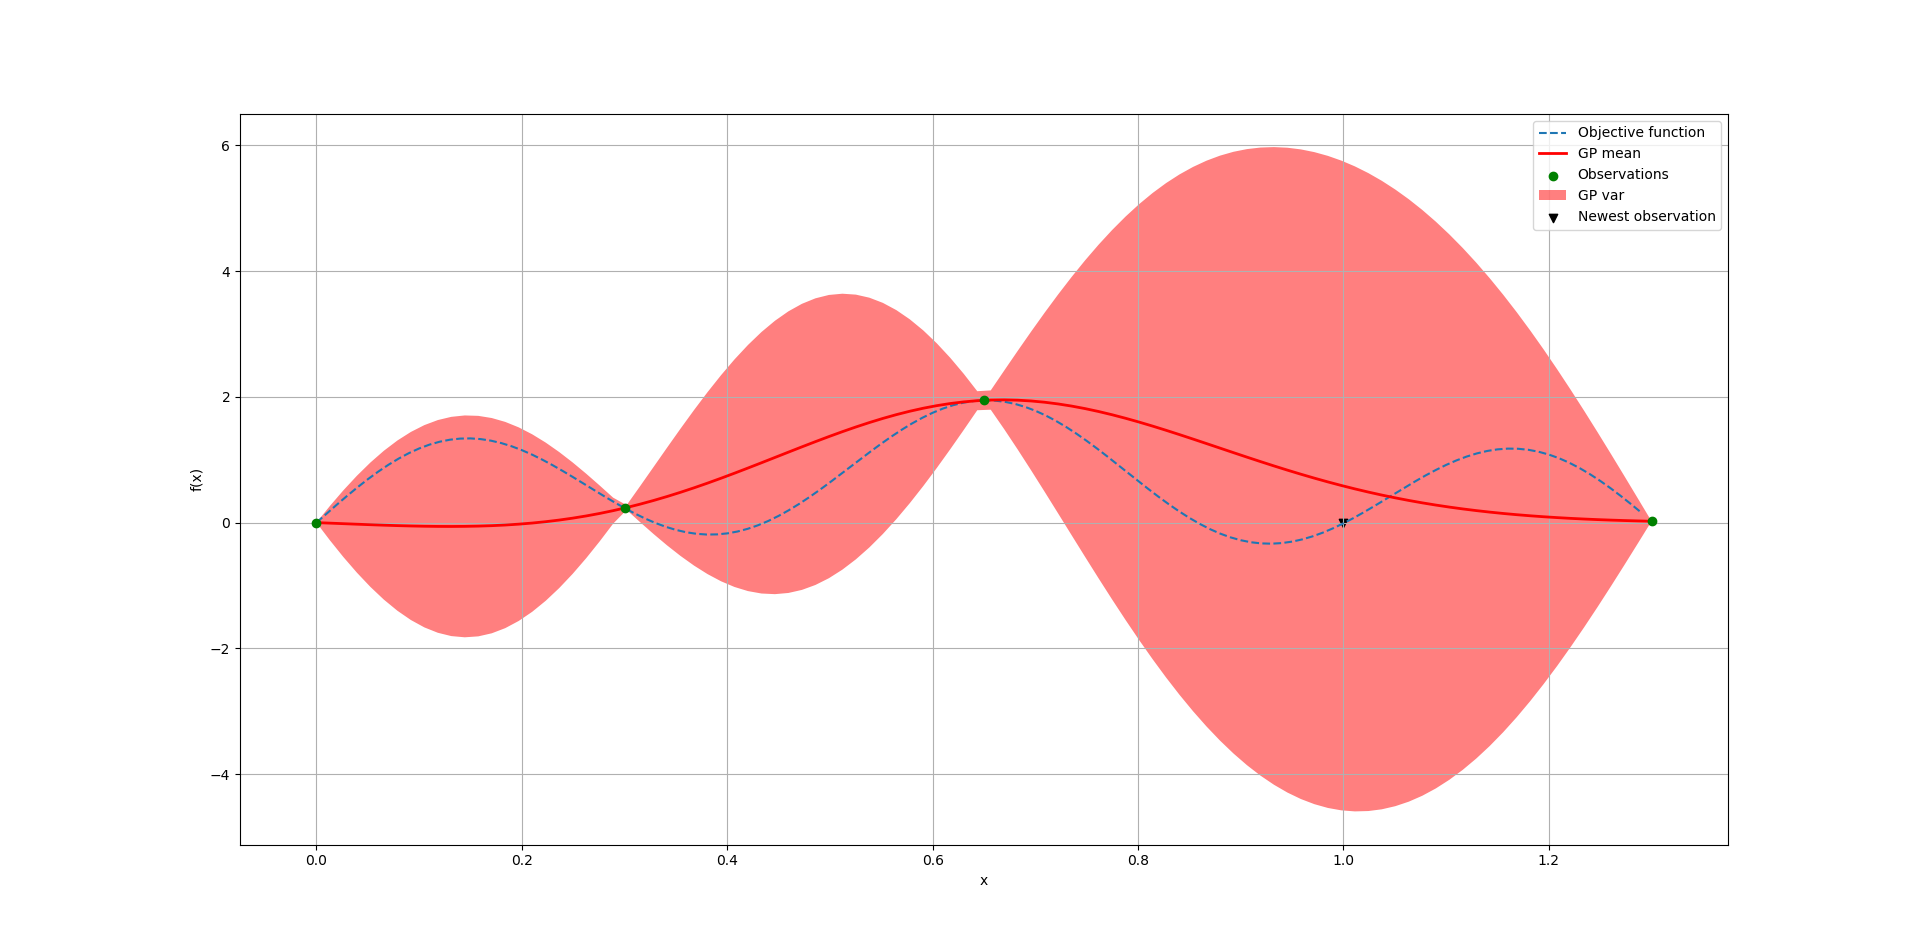
\includegraphics[width=\linewidth]{w06_hpo_bo/images/intro_images/BOLoop_2.png}}
    \only<3>{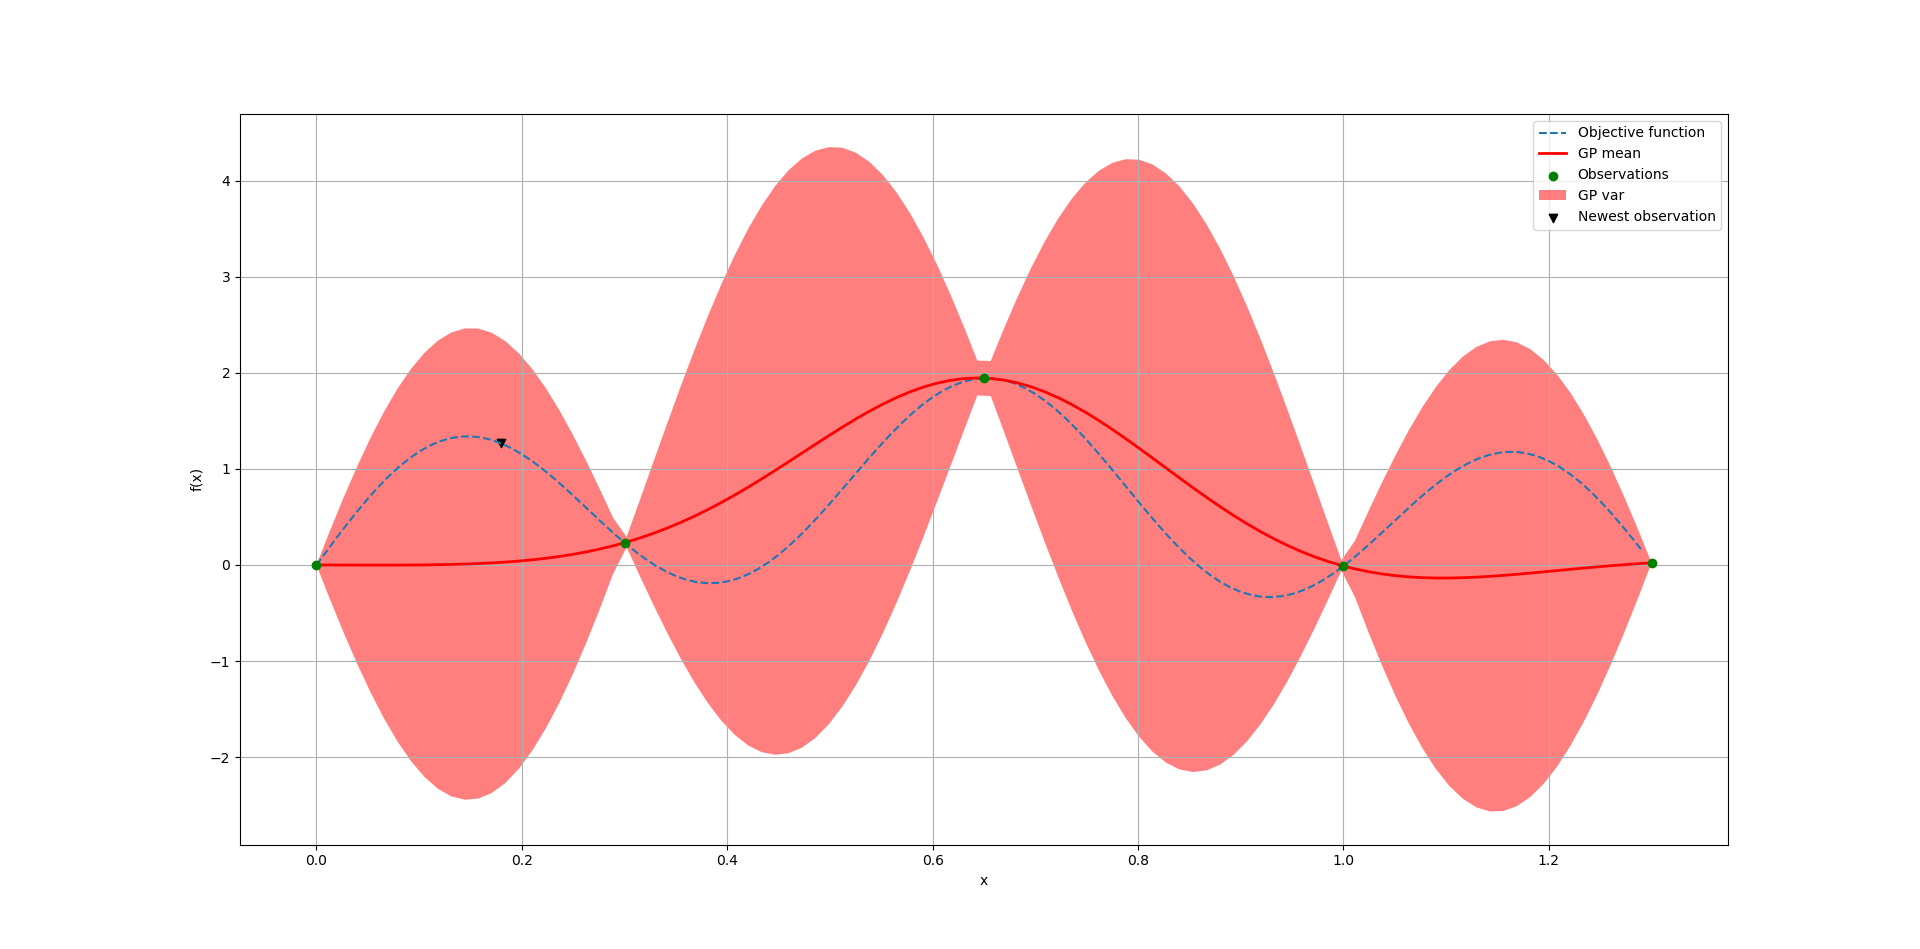
\includegraphics[width=\linewidth]{w06_hpo_bo/images/intro_images/BOLoop_3.png}}
    \only<4>{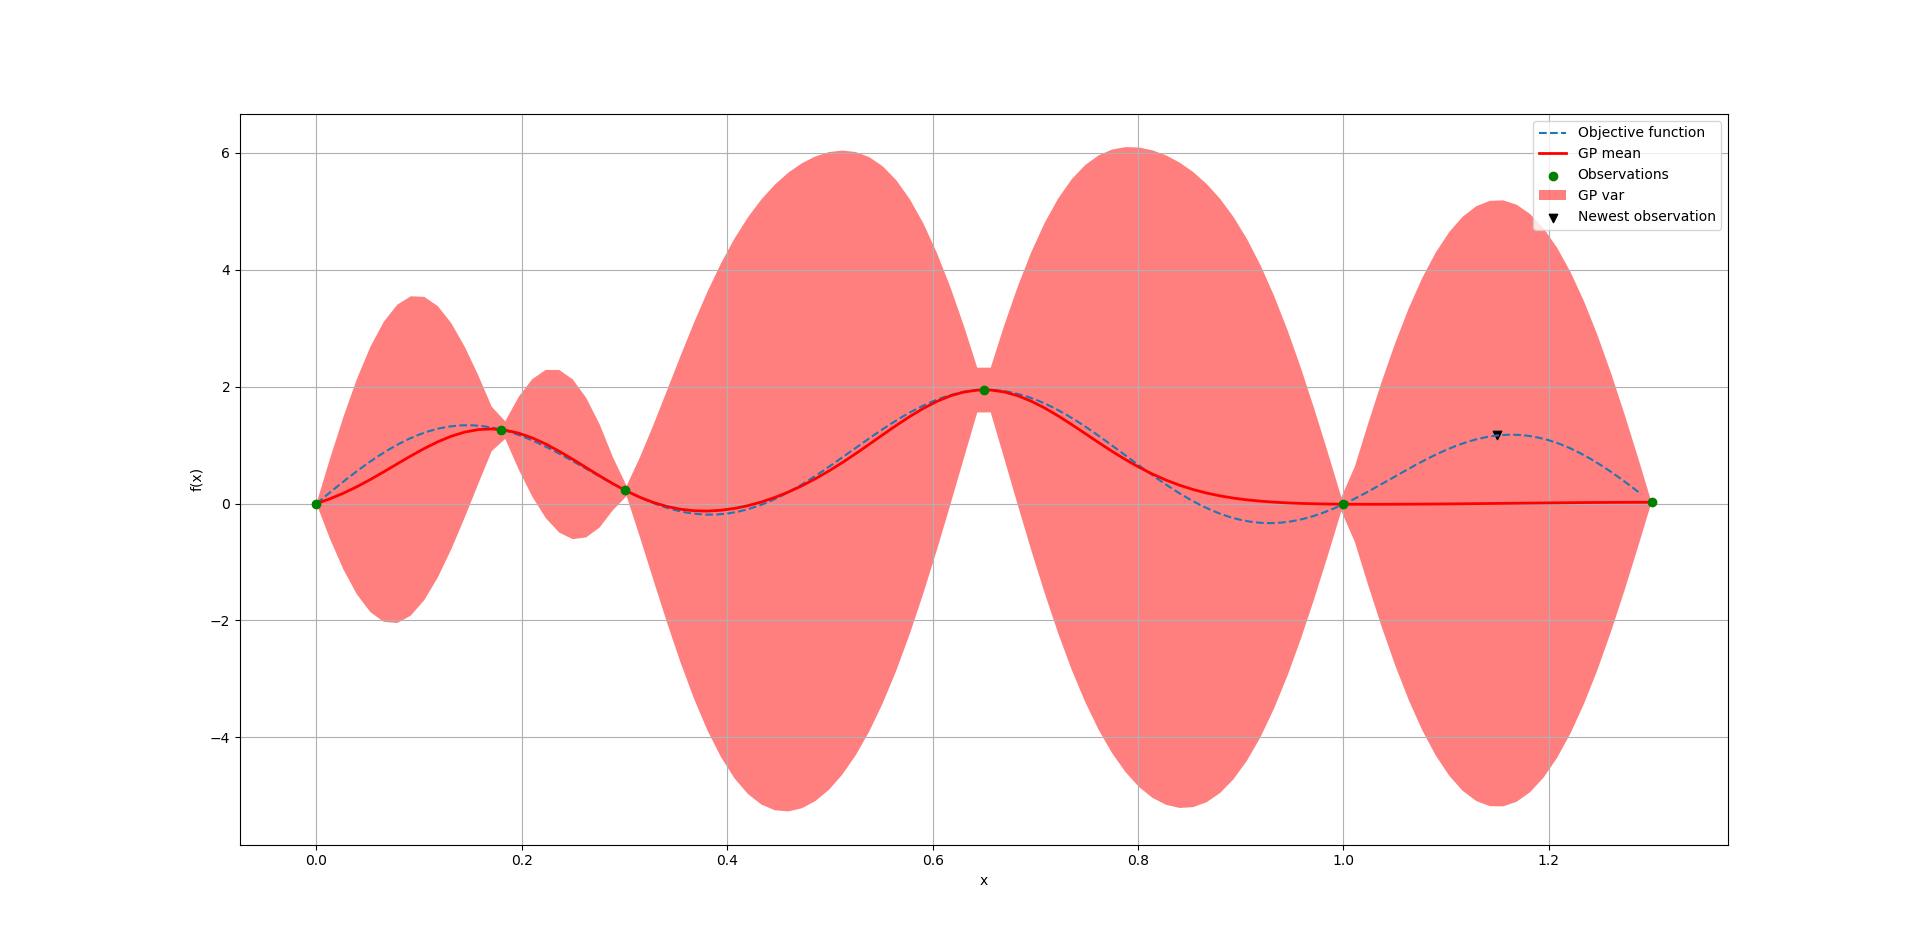
\includegraphics[width=\linewidth]{w06_hpo_bo/images/intro_images/BOLoop_4.png}}
    \only<5>{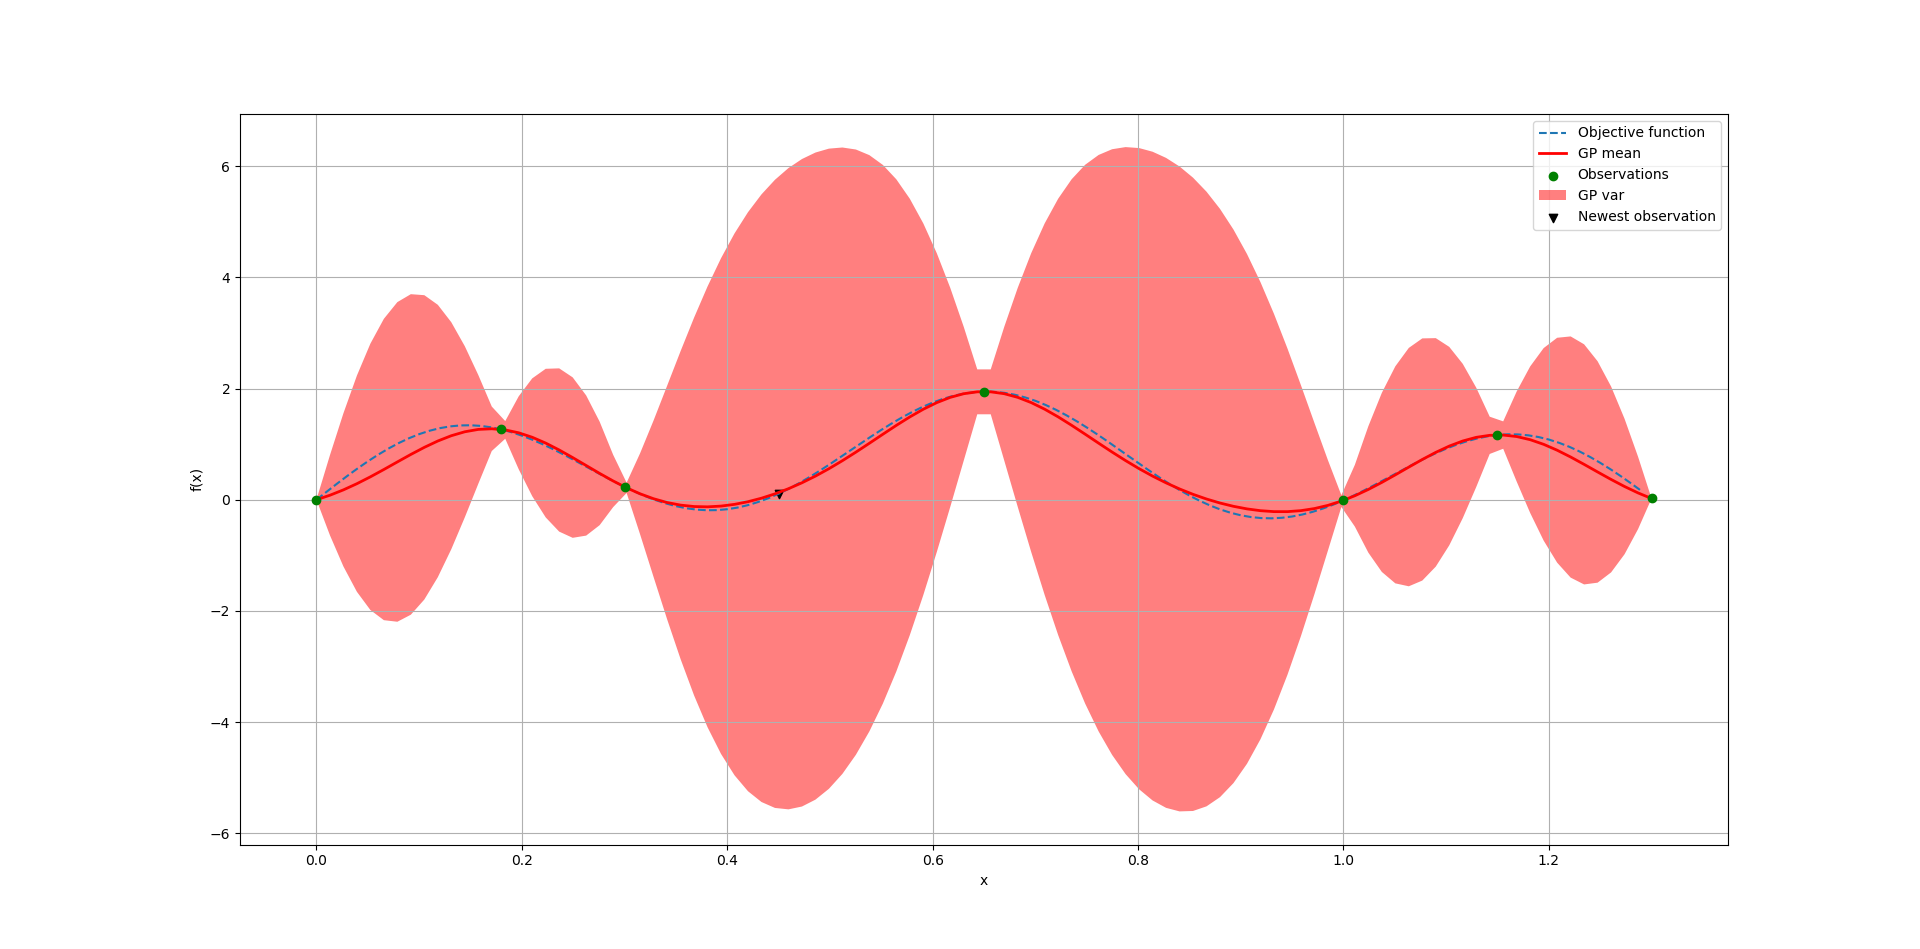
\includegraphics[width=\linewidth]{w06_hpo_bo/images/intro_images/BOLoop_5.png}}
    \only<6>{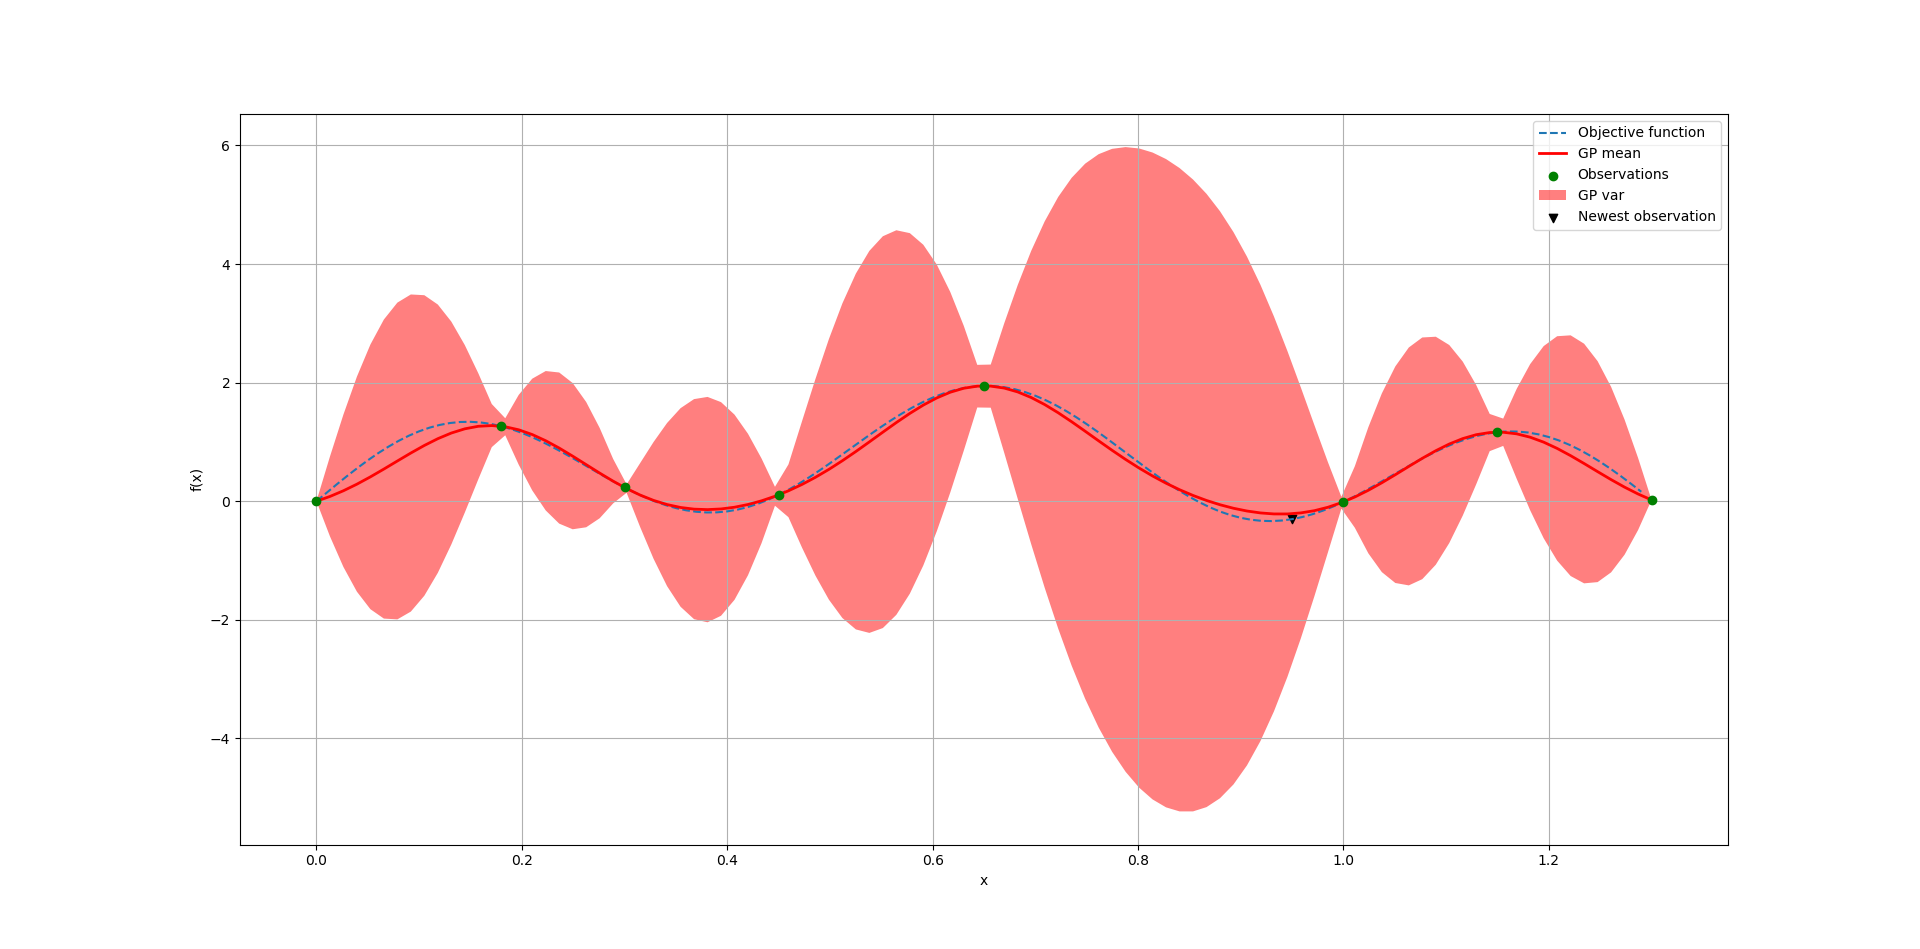
\includegraphics[width=\linewidth]{w06_hpo_bo/images/intro_images/BOLoop_6.png}}
    \only<7>{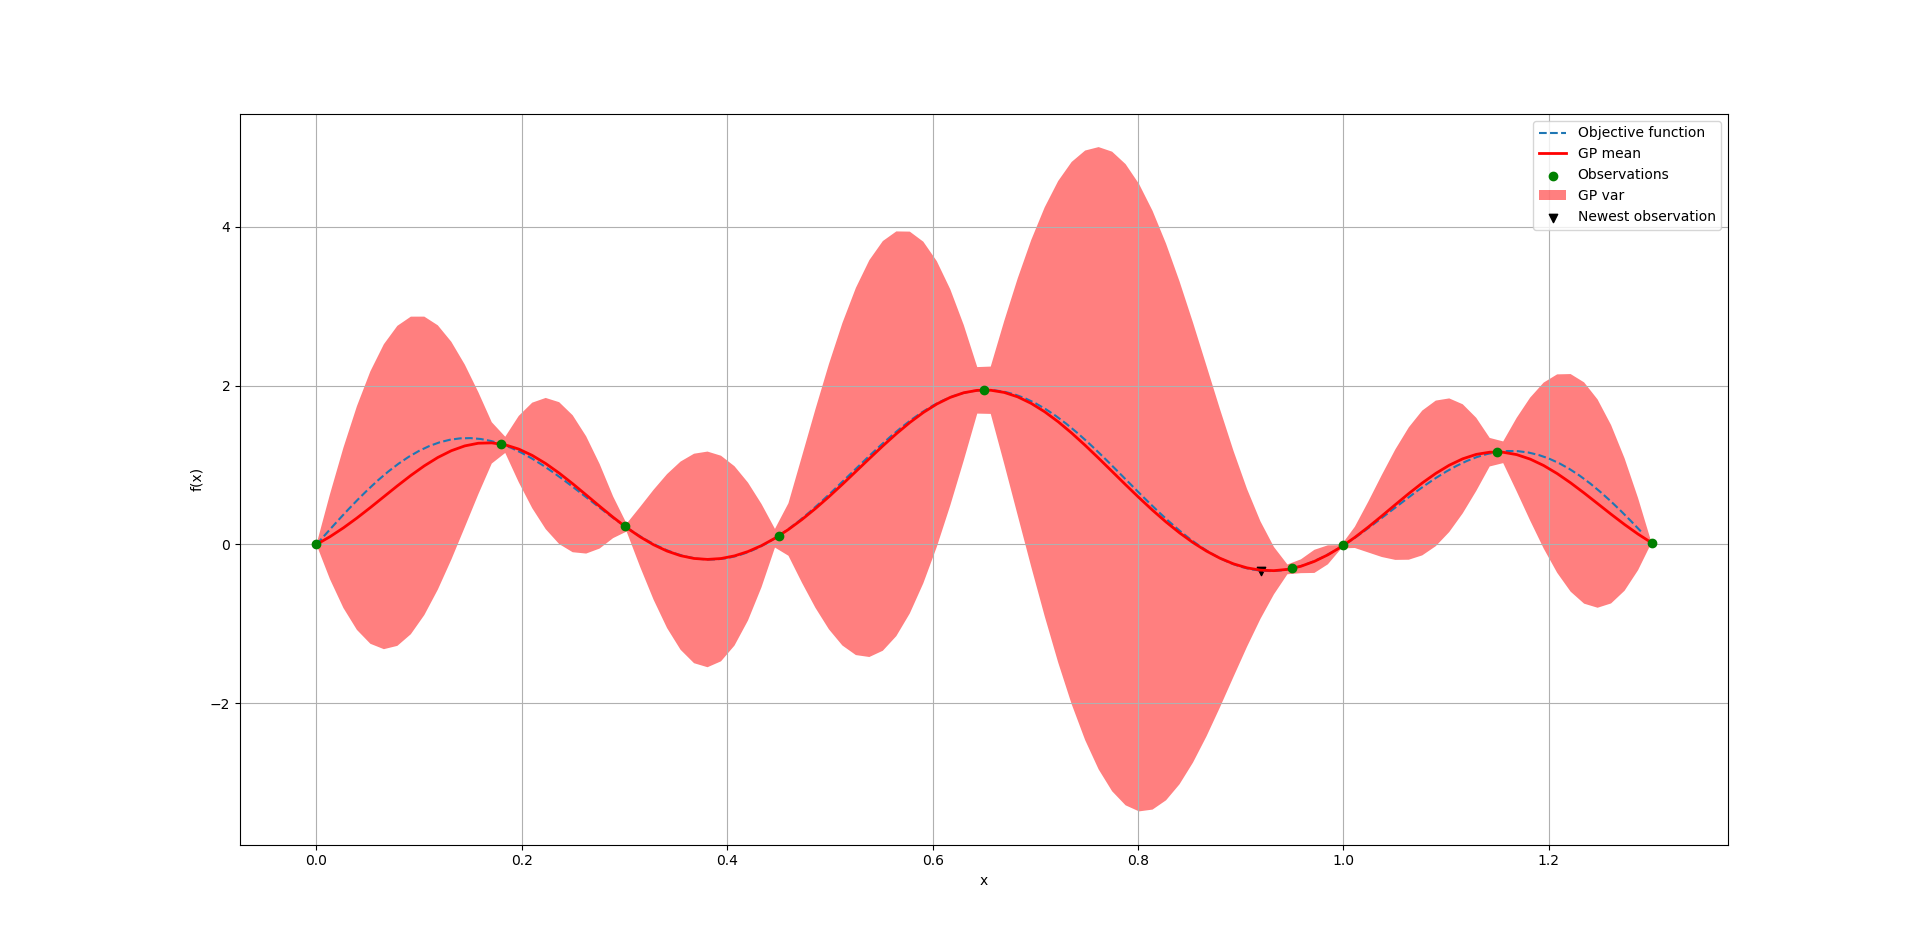
\includegraphics[width=\linewidth]{w06_hpo_bo/images/intro_images/BOLoop_7.png}}
    \only<8>{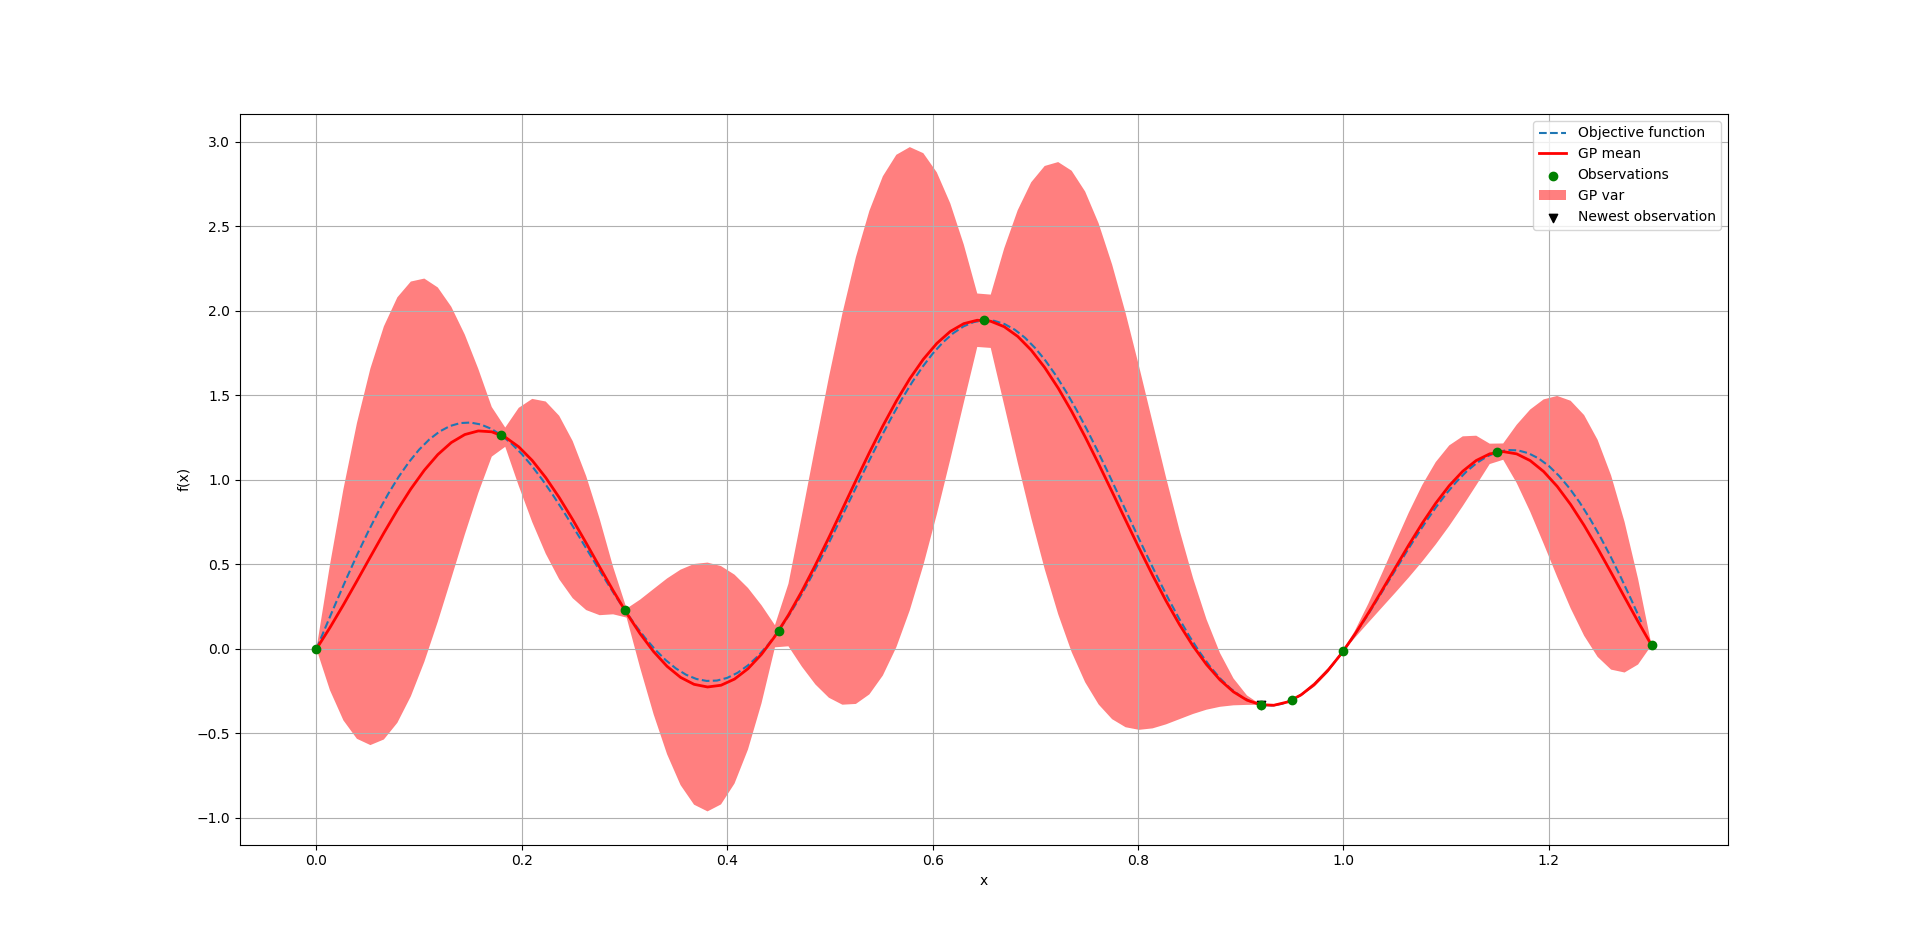
\includegraphics[width=\linewidth]{w06_hpo_bo/images/intro_images/BOLoop_8.png}}

\end{figure}


\end{frame}

%-----------------------------------------------------------------------
%----------------------------------------------------------------------
\begin{frame}[c]{Surrogate modelling}
\framesubtitle{General idea}
\begin{itemize}
    \item Use a surrogate model of the expensive function $\cost$ as a cheap-to-evaluate proxy.
    \begin{itemize}
        \item Use a probabilistic model with well-calibrated uncertainty predictions.
    \end{itemize}
    \pause
    \item Define a utility function to guide the search for new data points.
    \pause
    \item Use the optimization of the utility function as a decision procedure to provide inference on where to evaluate next.

\end{itemize}




\end{frame}

%-----------------------------------------------------------------------